\documentclass[a4paper,top=25mm,bottom=25mm,12pt,pdftex,halfparskip,twoside,openany,bibtotoc,numbers=noenddot]{scrbook}

\raggedbottom

\usepackage{fancyhdr}

\usepackage[utf8]{inputenc}
\usepackage{wrapfig}
\usepackage[pdftex]{graphicx}
\usepackage{caption}
\usepackage{subcaption}
\usepackage{eso-pic}
\usepackage{array}
\usepackage{pgfplots}
\usepackage{tabularx}
\usepackage{makecell}
\usepackage{multicol}
\usepackage{xcolor}
\usepackage{float}
\usepackage{enumitem}
\usepackage{listings}
\usepackage[toc,page]{appendix}
\usepackage[english]{babel}
\usepackage[backend=biber, style=numeric, natbib=true, hyperref=true]{biblatex}

\usepackage{todonotes}

\addbibresource{thesis.bib}

\linespread{1.25}

% chapters, numbering
\newcommand{\xchapter}{\stepcounter{chapter}\setcounter{section}{0}\addchap}

% tables
\renewcommand\theadalign{bc}
\renewcommand\theadfont{\bfseries}
%\renewcommand\theadgape{\Gape[4pt]}
\setlength{\tabcolsep}{4pt}
\setlength{\belowcaptionskip}{4pt}

\graphicspath{{img/}}

\fancypagestyle{plain}{%
	\fancyhf{}%
	\fancyfoot[LO,RE]{\thepage}%
	\renewcommand{\headrulewidth}{0pt}
}

\definecolor{gray}{rgb}{0.4,0.4,0.4}
\definecolor{darkblue}{rgb}{0.0,0.0,0.6}
\definecolor{cyan}{rgb}{0.0,0.6,0.6}
\definecolor{green}{rgb}{0,0.6,0}
\definecolor{mauve}{rgb}{0.58,0,0.82}

\lstset{
  basicstyle=\ttfamily,
  columns=fullflexible,
  showstringspaces=false,
  captionpos=b,
  commentstyle=\color{gray}\upshape,
  keywordstyle=\color{blue},       % keyword style
  stringstyle=\color{mauve},
}

\lstdefinelanguage{XML}
{
  morestring=[b]",
  morestring=[s]{>}{<},
  morecomment=[s]{<?}{?>},
  stringstyle=\color{black},
  identifierstyle=\color{darkblue},
  keywordstyle=\color{cyan},
  morekeywords={xmlns,version,type,name,as,id,style,x,y,width,height}% list your attributes here
}

% define medatata
\def\MOrg{Leopold-Franzens-University Innsbruck}
\def\MInstitution{Department of Computer Science}
\def\MGroup{Distributed and Parallel Systems Group}
\def\MTitle{High-Level Modeling and Low-Level Adaptation of Serverless Function Choreographies}
\def\MAuthor{Benjamin Walch\\ \small 01518922}
\def\MSupervisor{Sashko Ristov, PhD}
\def\MDate{\today}

\begin{document}

\frontmatter
\pagestyle{empty}

\begin{titlepage}
\rule{0mm}{1mm}

\begin{multicols}{2}[\columnsep2em] 
	\includegraphics[width=6cm]{uibk-logo}
	\columnbreak
	\begin{flushright}
		\Large{\textsf{\MOrg}}
	\end{flushright}
\end{multicols}

\begin{flushright}
	{\large \MInstitution\\}
	{\large \MGroup}
\end{flushright}

\vspace*{1.5cm}

\begin{center}
	{\LARGE\bf \MTitle}
	\vskip 2.25cm
	\Large \textbf{Bachelor Thesis}
	\vskip 2.25cm
	{\Large \MAuthor}
	\vskip 1.5cm
	{\large Supervisor: \MSupervisor}   
	\vfill
	{\large Innsbruck, \MDate}
\end{center}
\AddToShipoutPicture{
	\put(-55,55){
		\parbox[b]{\paperwidth}{
			\hfill \includegraphics[scale=0.35]{uibk-watermark}
		}
	}
}
\end{titlepage} 

\ClearShipoutPicture

\clearpage

\section*{Declaration}

By  my  own  signature  I  declare  that  I  produced  this  work  as  the  sole author, working independently, and that I did not use any sources and aids other than those referenced in the text. All passages borrowed from external sources, verbatim or by content, are explicitly identified as such.

I consent to the archiving of the bachelor thesis at the institute / faculty:

\vspace{1.8cm}

\parbox{6cm}{
	\hrule
	\strut \centering\footnotesize Date
} \hfill
\parbox{6cm}{
	\hrule
	\strut \centering\footnotesize Signature
}

\clearpage

\thispagestyle{plain}

\vspace{2.5cm}
\begin{center}
\textbf{Abstract}
\end{center}

Serverless computing has rapidly developed into a generally accepted cloud computing paradigm in recent years.
Based on serverless computing, \textit{Function-as-a-Service} (FaaS) emerged as a popular concept, in which pieces of code can be executed in the cloud using \textit{serverless functions}. Complex applications can be described using serverless functions in a \textit{serverless workflow}, enabling them to be deployed and executed in the cloud.
However, even with supportive tools, building serverless workflow applications is a difficult, time-consuming task, mainly reserved for developers.
Domain experts, who are well versed in their field would be best suited for creating business logic, but they generally are not familiar with serverless technologies.\\
A large number of providers followed the serverless trend, which resulted in a variety of tools and platforms for creating and executing serverless workflows, but none of them are compatible with each other.

The \textit{Abstract Function Choreography Language} (AFCL) was created as a platform-independent specification for describing serverless workflows at a high abstraction level. AFCL not only solves the problem of provider lock-in, but also overcomes weaknesses of current FaaS platforms. Still, AFCL workflows need to be created in a manual and time-consuming process: Either by writing YAML manually, or by writing Java code utilizing the AFCL Java API.

This thesis introduces AFCL ToolKit, which facilitates modeling of AFCL workflows, especially for non-developers. It allows the user not only to compose, but also to load, display, modify and export AFCL workflows. In addition, the developed system also offers adaptation of AFCL workflows at low-level by optimising workflows.

The results show the benefit of the system: Significant speedup in workflow development, minimization of human errors and availability of AFCL to non-developers.

\tableofcontents

\listoffigures

\listoftables

\mainmatter
\pagestyle{fancy}

\renewcommand{\chaptermark}[1]{%
	\markboth{\thechapter.\ #1}{}
}

\fancyhead{}
\fancyhead[LO]{\leftmark}
\fancyhead[RE]{\rightmark}
\fancyfoot{}
\fancyfoot[LO,RE]{\thepage}

\label{chap:introduction}
\chapter{Introduction}

"Run code, not Servers" is a recent term in the cloud computing world.
With the rise of serverless technologies during the last few years, \emph{Function-as-a-Service} (FaaS) has become increasingly popular. This cloud computing concept offers new advantages for software development: very high flexibility, nearly unlimited scalability and pay-per-use pricing. Entire programs can be defined in workflows by connecting serverless functions with data- and control-flow. Such serverless workflow applications, or \textit{function choreographies} (FCs), can be executed using serverless technology in the cloud.

However, each FaaS provider has its own definitions on how FCs are expressed in their environment, as well as different pricing models, limits and quotas. Thus, FCs from one system are not compatible with another, which means, the user is bound to a specific provider (provider lock-in), if they want to reuse an FC.

The creation of FCs would be the most efficient, if it could be done by domain experts who know their field best. But they usually lack the necessary know-how for serverless technology. Even though many FaaS providers offer tools which can support the creation of FCs in their environment, in most cases a software developer is still needed. And even for developers, this task can be tedious and time-consuming.

For current FaaS providers\footnote{\label{note:checked-providers}checked providers: AWS Step Funtions, Google Cloud Functions, IBM Cloud Functions and Microsoft Azure Functions}, specifying an FC is mainly a manual process by writing JSON, YAML or JavaScript into text files.
Although systems like AWS Step Functions or IBM Cloud Functions offer visualization of existing FCs, heir creation is still a manual process.
There is no question that manual processes are often a point of failure due to human error. The larger an FC description is, the more likely typos or other errors are.

\clearpage

The Distributed and Parallel Systems group of the University of Innsbruck developed a specification for describing FCs at a high abstraction level. This specification is called \emph{Abstract Function Choreography Language} (AFCL) and its main purpose is to overcome weaknesses of current FaaS platforms - one being the incompatibility of FCs between different providers.

With the possibilities of AFCL, the execution of an FC - or parts of it - could be distributed onto multiple providers. This is especially useful when the number of iterations of a concurrent loop is beyond the maximum number of concurrent function invocations allowed by the FaaS provider. To be able to scale independently of this limitation, the concurrent execution of all iterations of the loop could be distributed over multiple FaaS systems.
This distribution of the execution of an FC can also save costs and may increase performance.
To achieve this, manual adaptations depending on the distribution type of the FC are needed. Such adaptations can be even be more time-consuming than the creation of FCs; but generally the same problems apply as to the creation of FCs.

Castro et al. mention that, "One of the major challenges slowing the adoption of serverless is the lack of tools and frameworks" \cite{articles-rise-of-serverless-castro}.

Therefore, the goal for this thesis is to develop a system, which facilitates development of AFCL FCs and focuses on business logic.
The system should also provide an interface for performing various adaptations on FCs at low-level.

This thesis fulfills the above goals and overcomes the aforementioned problems.
With the developed system, which we will refer to as "AFCL ToolKit" in the text below, it is possible for non-developers to create an FC in less time than it would have taken a developer to write the FC in AFCL.
Unlike most of the current tools, AFCL ToolKit facilitates the creation of FCs by providing a graphical user interface (GUI) where the user can model FCs being visualized directly using drag and drop. Loading, displaying and editing of existing AFCL FCs is also supported.
FCs created with AFCL ToolKit are guaranteed to be valid in AFCL, which minimizes human errors.
AFCL ToolKit also ships with an interface for performing adaptations on FCs at low-level, based on specific inputs.

It is assumed that concrete implementations of serverless functions are already developed and deployed to a FaaS provider.

\newpage

In the next chapter \ref{chap:background}, we will give background information on topics related to this thesis. After that, in chapter \ref{chap:afcl-toolkit}, a closer look at the system architecture and design of AFCL ToolKit is given, before the application's user interface is presented and explained in chapter \ref{chap:user-interface}.

Finally, we evaluate AFCL ToolKit and clarify its benefits to the developed system in chapter \ref{chap:evaluation}, before moving on to a discussion about the AFCL API in chapter \ref{chap:discussion}.

\chapter{Background}
\label{chap:background}

This chapter contains important details on the terms and technologies used in this thesis and helps the reader to better understand the further topics.\\
First of all, the serverless concept, in particular FaaS, serverless functions and serverless workflows are explained, before giving a brief overview about AFCL. The tools and technologies used for development are also presented to readers who are not yet familiar with them.

\section{Serverless computing}

Serverless computing is widely known as an event-driven cloud execution model.
In this model, the client provides the code  and the cloud provider manages the life-cycle of the execution environment of that code.
The idea is based on reducing the life span of the program to execute functionality in response to an event. Hence, the program's processes are born when an event is triggered and are killed after the event is processed \cite{inproceedings-serverless-beyond-the-cloud-kanso}.
Developers can completely focus on the program they need to run and not worry at all about the machine it is on or the resources it requires \cite{articles-going-serverless-savage}.
Castro et al. define serverless computing as follows: "Serverless computing is a platform that hides server usage from developers and runs code on-demand automatically scaled and billed only for the time the code is running" \cite{articles-rise-of-serverless-castro}.

The term "serverless" can be misleading though, as there are still servers providing these backend services, but all of the server space and infrastructure concerns are handled by the vendor. Serverless means that the developers can do their work without having to worry about servers at all \cite{online-what-is-serverless-cloudflare}.

\section{FaaS}

FaaS is a form of serverless computing, which is disrupting the way applications and systems have been built for decades. By abstracting infrastructure provisioning and deployment, user-provided functions can be invoked and executed remotely. The user only has to worry about development and triggering of the function. This serverless runtime has not only the advantage that it avoids costly pre-allocated or dedicated hardware, but also offers almost unlimited possibilities in scalability. FaaS systems are designed to allow a usage-based billing, what means the user will only be charged for resources required during execution.

\section{Serverless functions}
Serverless functions - or tasks - are single-purpose, mostly stateless, programmatic functions that are hosted on cloud infrastructure. This infrastructure is provided through a FaaS platform. They are event-driven and can be invoked through the internet, mainly using HTTP. Like conventional functions, they accept arguments and and return the result of the computation  - tthe difference being that this is done over a network.

\section{Serverless workflows}
On an abstract level, a workflow consists of a set of interdependent tasks that need to be executed to achieve a specific goal. A task within a workflow has the following properties: dependencies on the software or service used by the task to perform its computation (software flow), dependencies on data (data flow), and dependencies on other tasks (control flow) \cite{thesis-design-serverless-worfklow-system-eyk}.\\

A serverless workflow, also known as \textit{function choreography} (FC), is a complex workflow defined through the composition of serverless functions, connected by data- and control-flow. FCs make it possible to combine and reuse serverless functions in order to build more complex applications. 
FCs can declare whole applications - and using formats like YAML or JSON, they can be described in a text-based file.

As mentionend in the introduction, current FaaS providers handle the creation and management of FCs differently:
In AWS Step Functions, FCs are expressed in a JSON-based structure which defines a state machine.
In both IBM Cloud Functions and Google Cloud Functions, FCs can only be defined in a specific programming language.
Microsoft has Azure Logic Apps, which make creation of JSON-based FCs possible on a higher abstraction level through a GUI.
But for all of these providers, their FCs are not compatible with each other.
Scenarios for porting FCs to another FaaS provider aren't unlikely; reasons for (partially) moving FCs to another system could be cost or performance issues.
Let us consider an FC built with AWS Step Functions, which should be executed on IBM Cloud. 
To make that work, the FC has to be ported to the other platform to be compatible - in other words - it has to be recreated by a skilled programmer.

\section{AFCL}

This section gives the reader a brief overview on AFCL and its features. More detailed information about AFCL as well as the API documentation can be found at \cite{online-afcl-dps}.

The \emph{Abstract Function Choreography Language} (AFCL) was created to overcome weaknesses in current FaaS platform implementations. As the name indicates, this specification describes FCs at a high level of abstraction, forming a step on the way to cross-cloud execution.

The AFCL specification also has more extensive control-flow and data-flow constructs available than current FaaS providers offer, in terms of language features. Therefore, AFCL can not only eliminate the incompatibility of FCs between different providers (vendor lock-in), but also opens the door to execute an FC by distributing its computation over multiple FaaS providers.

To be able to actually execute such multi-cloud FCs, some further tools are needed: an Enactment Engine and a Scheduler, which are beyond the scope of this thesis.

\subsection{Overview}
AFCL is based on YAML\footnote{https://yaml.org} and ships with a schema\footnote{http://dps.uibk.ac.at/projects/afcl/files/schema/schema.yaml}. There exist two types of functions, base functions and compound functions, which can be connected by specifying control-flow and data-flow information. While base functions represent a single task, compound functions provide nesting - they can include some base functions or even other compound functions.

Base and compound functions have data input (dataIns) and data output (dataOuts) ports.
Data input can refer to another data output or data input of another function, by specifying the name in combination with the data output port of the other function.

\subsection{Control-flow}
In AFCL, base or compound functions are specified one after another, which means that they are executed sequentially. However, the following control constructs are introduced with AFCL: \texttt{sequence}; \texttt{if-then-else}; \texttt{switch}; \texttt{for}; \texttt{while}; \texttt{parallel}; and \texttt{parallelFor}.


\subsection{Properties and Constraints}

Additional, optional attributes for \texttt{dataIns} and \texttt{dataOuts} ports of a function, or for the function itself can be defined in \texttt{properties} and \texttt{constraints}. While those are simple key-value pairs accepting string values, AFCL has a few defined properties and constraints to specify concrete attributes like invocation type of a function, element index or data distribution information in loops.

% data-flow (dag based)
\subsection{Data-flow}
AFCL allows the expression of data-flow by connecting the source data ports of functions to the target data ports of functions. This offers support for more complex data-flow scenarios and might improve performance of the FC. A source data port can be the input data port of the whole FC, or a data port (input or output) of another function. So it is possible to even connect data ports of outer functions, with a a lower nesting level, to inner functions, with a higher nesting level. 

\section{Tools and Technologies}
\subsection{npm}

The \textit{node package manager}\footnote{https://www.npmjs.org} (npm) is the world's largest software registry, where open-source software packages of developers and companies are shared all over the world. Over the last few years, npm has become a de-facto standard for package management in JavaScript development.

\subsection{webpack}

\textit{webpack}\footnote{https://webpack.js.org} is a module bundler, its main purpose is to bundle JavaScript code for the usage in a browser. In particular, multiple modules (often hundreds of them) with dependencies [to each other] are processed and bundled into a few files. To be able to process other types of files than JavaScript or JSON, webpack offers the opportunity to configure a \textbf{loader}. In this application, the following loaders are configured:
\begin{itemize}
\item babel-loader, to transform ES and React JSX to browser-compatible JavaScript
\item sass-loader, to transform SASS to CSS
\item css-loader, to transform CSS to CommonJS
\item file-loader, to handle static resources like images and fonts
\end{itemize}

\subsection{ECMAScript}

The scripting language specification \textit{ECMAScript} (ES) was created to standardize JavaScript. With the release of ES6 (also known as ECMAScript 2015), features like class declarations, module imports and arrow function expressions became possible. After ES6, every year a new edition of the ECMAScript standard was finalized and released, offering new features. It is particularly worth highlighting here is the rest/spread operator feature which was released with ES9, as it was used a lot in this thesis.

\subsection{Babel}
Since current browsers only have partial support of ECMAScript, a \textit{transcompiler} or \textit{transpiler} is needed to transform the ECMAScript source code to JavaScript, which common browsers are capable of interpreting.
\textit{Babel}\footnote{https://babeljs.io} is an industry standard to transpile ES to common JavaScript or lower ES versions.

\subsection{SASS}

CSS, in its pure form, reaches its limits when one thinks about using variables, functions or nested rules. \textit{SASS}\footnote{https://sass-lang.com} is a stylesheet language, which is - similiar to ES - compiled to CSS and offers the aforementioned and other features.
A lot of CSS Frameworks also provide their source code in SASS, often served with a large variable set which makes customization easy.

\chapter{AFCL ToolKit}
\label{chap:afcl-toolkit}

This chapter gives the reader a detailed overview on the system architecture and the system design of AFCL Toolkit, including evaluations about technology decisions for specific tasks.

AFCL ToolKit is not designed to just visualize FCs described in AFCL, it's purpose is much more about having an overall system, in which different tools facilitate working with AFCL FCs.
The system is built such that further tools can be easily integrated as own components.\\
In context of this thesis, a system with the following main components was developed: A function repository, to store functions which will be used in the system; an editor, where the user can model FCs at a high level of abstraction; and a service, for performing adaptations on FCs at low-level.

%Figure \ref{fig:user-actions} shows the user actions which result out of the components described above.

%\begin{figure}[H]
%  \centering
%  \includegraphics[width=0.75\textwidth]{user-actions}
%  \caption{AFLToolKit features}
%  \label{fig:user-actions}
%\end{figure}

\section{System Architecture}
\label{sec:afcl-toolkit-architecture}

The overall system is built on top of two sub systems which are operating mostly decoupled from each other. On the one hand there is the backend, responsible for low-level operations as well as persistence of function data.\\
On the other hand is the frontend providing a GUI, which is responsible for user interaction, data visualization and file I/O.
Those two sub systems interact with each other by sharing JSON-serialized objects through an application programmable interface (API), which the backend provides and the frontend consumes.

\begin{figure}
  \centering
  \includegraphics{architecture}
  \caption{System architecture}
  \label{fig:system-architecture}
\end{figure}

\subsection{Frontend}

The frontend displays and controls the application's user interface and is accessible through a web browser. Its main component is the editor, where the user can compose and change FCs in a \textit{what-you-see-is-what-you-get} (WYSIWYG) manner.

\subsubsection{Editor}

By providing an editor which follows the WYSIWYG principle, modeling FCs at a high level of abstraction is possible.
In particular, FCs in the editor are presented to the user as a directed graph. Functions and control-structure are represented by the graph's nodes, while the edges define execution flow. Therefore, the editor also includes logic for graph drawing, visualization and layouting.\\
The user can create a new graph or edit the graph being visualized by drag and drop, while changes are constantly validated to ensure graph validity.
The modeling process is supported by additional features like change history (versioning), clipboard (copy-paste) and automatic layouting.

\subsubsection{Validation}
As mentioned before, validation takes place after changes on the graph were made. The graph is validated against explicit and implicit rules of AFCL.
For example, an explicit rule is, that in AFCL the name of a function must be unique.
An example for an implicit rule is that there must exist only one starting point in the graph. 

All details about validation and its constraints are described in section \ref{sec:graph-validation}.

\subsubsection{Encoding and decoding}
Encoding and decoding components control the conversion of graph data from a human-readable format (the graph visualization itself) into a machine-readable format (in this case XML) and vice-versa. The conversion is needed in order to enable other parts of the system to perform operations on the data.

\subsubsection{Input and output}

The frontend accepts YAML or JSON files for loading existing FCs expressed in AFCL. When opening a file, its contents is decoded into an intermediary representation - capable of being visualized as a graph. When saving, the visualization of the current graph's state is encoded to XML, and sent to the user by offering a download. The XML file includes all necessary information which is needed to load or restore the current graph's state later. FCs being edited can also be exported into AFCL files (YAML, JSON) which is the result of a conversion on the backend side of the encoded current graph representation (XML) to AFCL.

All features of the web-based user interface are described in detail in section \ref{chap:user-interface}.

\subsection{Backend}

The main purpose of the backend is to perform operations on FCs at low-level. These operations include the conversion of graph XML data delivered from the frontend, as well as more complex FC modifications. The persisting of function data is also covered by the backend.

\subsubsection{Function repository}

The storing of function data is abstracted from the user and persisting of the data is handled internally.
The repository implemented in this thesis, stores the serialized data into a file. This could be easily replaced with any other implementation, for example an implementation which stores the data in an external database management system (DBMS).

\subsubsection{Adaptation}

The backend provides a service for performing low-level FC adaptations, which is accessible through an API.
The concrete adaptation for FCs developed in this thesis is to divide one concurrent loop into multiple concurrent loops which run in parallel.
Figure \ref{fig:workflow-adaptation} visualizes the core part of this adaptation in its simplest form.\\
This service can be either consumed by the user through the user interface, or by other systems through the API. For example, a scheduler, which is not part of this thesis, would decide to divide a large parallel loop and uses the API of the backend to do this adaptation.

\begin{figure}[H]
\centering
\begin{subfigure}{.28\textwidth}
  \centering
  \includegraphics[width=.8\linewidth]{adaptation-before}
  \caption{before adaptation}
\end{subfigure}
\begin{subfigure}{.54\textwidth}
  \centering
  \includegraphics[width=.8\linewidth]{adaptation-after}
  \caption{after adaptation}
\end{subfigure}
\caption{FC adaptation example}
\label{fig:workflow-adaptation}
\end{figure}

\subsubsection{Interfaces}

For the communication with other parts of the system (the frontend), or with external systems (e.g. a scheduler), the backend includes a web server, which is used to expose the backend's API through the network. For example, requests initiated by the frontend for converting XML graph representations into AFCL FCs are handled by that API. The result of the operation is then returned to the frontend. A similiar procedure applies for function data, where read and write requests initiated by the frontend are processed and returned.

\clearpage

\section{System Design}

Beyond the overall system architecture, we will now look deeper into the system design.
This  section  focuses on how the implementation of the system was achieved.\\
Care has been taken to ensure that all used libraries in the project are open source.

\subsection{Frontend}

The frontend is built as a web application with HTML, CSS and JavaScript.\\
The JavaScript library \textit{React}\footnote{https://reactjs.org} is primarily used to build the user interface. One of the benefits when using React is that the data model displayed to the user typically maps very well to UI components \cite{online-react-thinking-in-react}.

\subsubsection{Stack}

The base forms npm, which is used to manage and resolve dependencies.  Webpack can be seen as the main part of the stack, which orchestrates transpiling and bundling all sources and assets into single files by utilizing so-called loaders.

Babel is used as such a webpack loader for transpiling the ECMAScript and React JSX source code to browser-compatible JavaScript.
The same applies for the CSS extension SASS, which is also integrated with a loader, and is used to make the process of styling the user interface more efficient.

webpack also executes some optimization plugins when building for production, which minimizes the size of the final bundle.

\begin{figure}[H]
  \centering
  \vspace{0.8cm}
  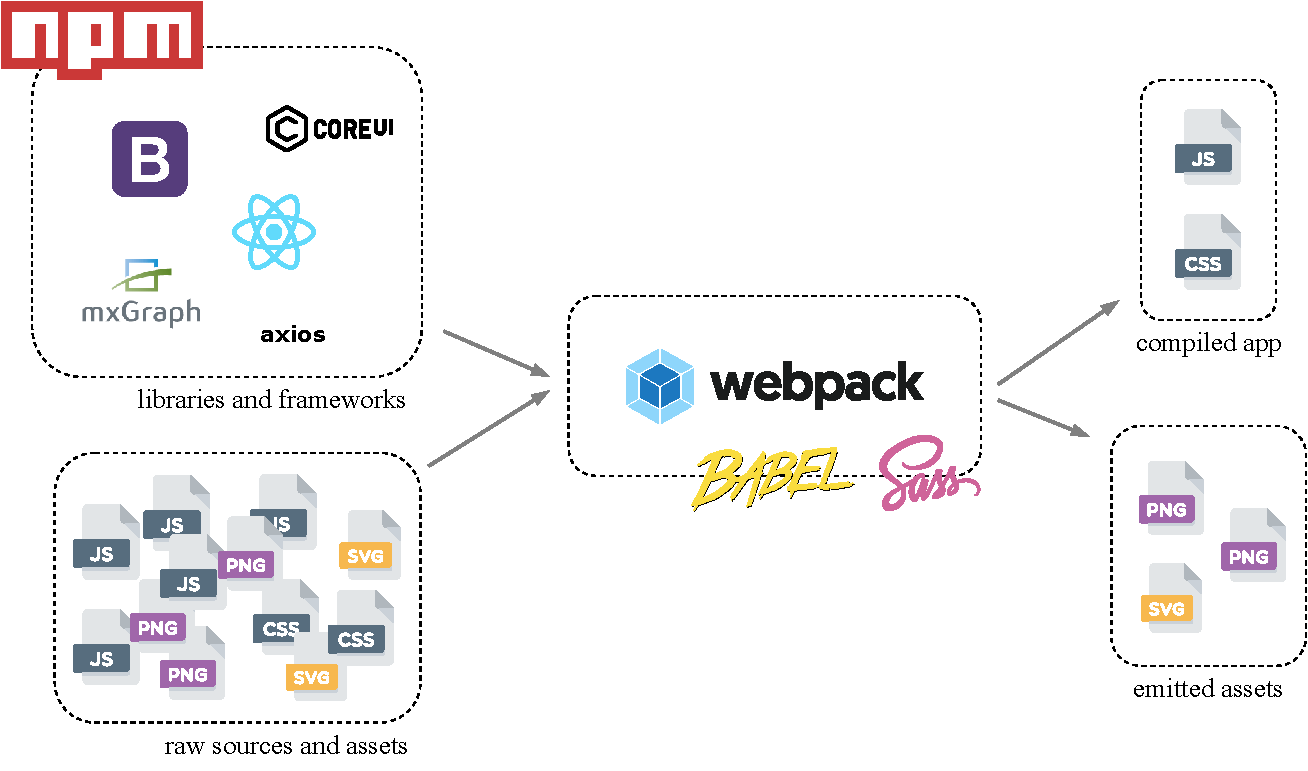
\includegraphics[width=0.8\textwidth]{frontend-setup}
  \caption{frontend stack}
\end{figure}

\subsubsection{Communication with the backend}
\textit{axios}\footnote{https://github.com/axios/axios/}, which is a JavaScript networking library, is used to communicate with the backend, by sending HTTP requests to the corresponding backend endpoints.

\subsubsection{Data model}

All Java classes of the AFCL Java API \citep{online-afcl-dps} have been ported to ECMAScript, to have all classes and properties also available in the frontend. Although plain JavaScript objects would also do the job, this adds a kind of type-safety to the ECMAScript sources and improves readability of the code. Also, the data exchange with the backend and the encoding of the visual graph representation benefit from this approach, since the XML node names map to constructor names.

\subsubsection{Graph drawing}

an FC can be represented as a directed acyclic graph (DAG). DAG's are conventional models to present workflows, where nodes are tasks and edges are communications between tasks.

At the time of implementation, the JavaScript library mxGraph was the best choice for the graph visualization and modification.\footnote{see \ref{sec:graph-alternatives} to learn why}
It has an outstanding documentation, enriched with a lot of demos and example code which show many use cases and extensive features, as well as a powerful production-grade example.\footnote{https://draw.io}\\
The authors of mxGraph state:\\
\begin{quote}
``mxGraph is pretty much feature complete, production tested in many large enterprises and stable for many years. We actively fix bugs and add features [...].''
\end{quote}

\subsubsection{Graph model}

In mxGraph, vertices and edges are represented by an \texttt{mxCell} model, which holds information about behaviour and appearance. Position and dimension of a \texttt{mxCell} are defined in a associated \texttt{mxGeometry} object. Figure \ref{fig:mxcell-model} shows the \texttt{mxCell} model with some properties and the relation to \texttt{mxGeometry}. The \texttt{mxCell} class has been subclassed in a custom class \texttt{Cell}, in order to add a \texttt{type} property and some additional logic.

\begin{figure}[H]
  \centering
  \includegraphics[]{mxCell}
  \caption{\texttt{mxCell} model}
  \label{fig:mxcell-model}
\end{figure}

In the further text, the term \textit{cell} refers to the visual element (which can be a vertex or an edge) in the graph, which is always represented by an instance of \texttt{Cell}, respectively.

\subsubsection{Graph context}

A \textit{user object} can be associated with a \texttt{mxCell} through the \texttt{value} property. User objects give the graph its context, they store the business logic associated with the visual part. For simple cases, the user object may be a string to display the cell's label. In more complex applications, the user object may be an object and some property of that object will generally be the label that the visual cell displays \cite{manuals-mxgraph-user-manual}.\\
For cells which represent an AFCL construct, the associated user object is an instance of the corresponding ported AFCL class.\\
For auxiliary cells like start-, merge-, or end cells, the associated user object is either just a string or none. Figure \ref{fig:graph-context-user-obj} presents a minimal graph example, indicating cell types and the corresponding type of the associated user object.

\begin{figure}[h]
  \centering
  \vspace{1.5cm}
  \includegraphics[]{cell-user-objects}
  \caption{A graph's cells and associated user objects}
  \label{fig:graph-context-user-obj}
\end{figure}

\newpage

Table \ref{tbl:frontend-impl-shapes} shows the implemented \texttt{Cell} types which are used as visual elements to represent a node in the graph. As well as a short description, the type of the associated user object is indicated.

\begin{table}[H]
\centering
\def\cellgape{\Gape[4pt]}
\def\arraystretch{2}
\begin{tabular}{ |c|c|c| } 
\hline
\thead{Cell} & \thead{Description} & \thead{User Object} \\
\hline
\makecell{
\includegraphics[width=32pt,height=32pt]{cell-start} \\ \textsf{Start}}  & Defines the FC's entry point & \makecell{\texttt{String} \\ \small(for the label)} \\
\hline
\makecell{\includegraphics[width=32pt,height=32pt]{cell-end} \\ \textsf{End}}  & Defines the FC's termination & \makecell{\texttt{String} \\ \small(for the label)} \\
\hline
\makecell{
\includegraphics[width=52pt,height=28pt]{cell-function} \\ \textsf{Function}}  & An atomic function & \texttt{AtomicFunction} * \\
\hline
\makecell{\includegraphics[width=32pt,height=32pt]{cell-ifthenelse} \\ \textsf{If-Then-Else}}  & A mutual exclusive condition & \texttt{IfThenElse} * \\
\hline
\makecell{
\includegraphics[width=32pt,height=32pt]{cell-switch} \\ \textsf{Switch}}  & A multi condition & \texttt{Switch} * \\
\hline
\makecell{
\includegraphics[width=32pt,height=24pt]{cell-merge} \\ \textsf{Merge}}  & An element for merging previous branches & \makecell{\texttt{null} \\ \small(none)} \\
\hline
\makecell{
\includegraphics[width=50pt,height=32pt]{cell-compound} \\ \textsf{Parallel}}  & \makecell{A container, where each child cell\\ is meant to be executed in parallel.} & \texttt{Parallel} * \\
\hline
\makecell{
\includegraphics[width=50pt,height=32pt]{cell-compound} \\ \textsf{ParallelFor}}  & \makecell{A container, where each child cell\\ is meant to be executed in a parallel for loop.} & \texttt{ParallelFor} * \\
\hline
\end{tabular}
\caption{Implemented Cells, *: AFCL Object}
\label{tbl:frontend-impl-shapes}
\end{table}

\newpage

\subsubsection{Graph validation}
\label{sec:graph-validation}

The visual representation of an AFCL FC has to meet the constraints of a DAG, as well as additional constraints to ensure compliancy of the FC to AFCL. An example would be the uniqueness of a function's name or that an AFCL FC has a starting and termination point. Compound AFCL constructs are designed to enclose its child functions, which is visualized in the same way in the graph. As a result, it has to be ensured that there exists no direct connection from a cell inside a container to a cell outside that container.
This leads to the following constraints below:

\begin{itemize}
    \item There exist no cycles
    \item Each edge has an orientation
	\item There exists exactly one \textsf{Start}
	\item There exists exactly one \textsf{End}
    \item Every \textsf{Cell} has a path to \textsf{Start}
    \item Every \textsf{Cell} has a path to \textsf{End}
	\item \textsf{Function}, \textsf{If-Then-Else}, \textsf{Switch}, \textsf{Parallel}, \textsf{ParallelFor} and \textsf{End} have exactly one incoming edge
	\item \textsf{Start}, \textsf{Function}, \textsf{Parallel}, \textsf{ParallelFor} and \textsf{Merge} have exactly one outgoing edge
	\item \textsf{If-Then-Else} has exactly two outgoing edges (then, else)
	\item \textsf{Switch} has multiple outgoing edges (the cases)
	\item \textsf{Merge} has multiple incoming edges
	\item Both \textsf{Cell}s taking part in a direct connection, must have the same nesting level, what means they must have the same parent cell
	\item A \textsf{Cell}'s label has to be unique in the graph
\end{itemize}

All the constraints above are enforced at different events. The validation is triggered when editing, especially when adding and connecting vertices, and when saving or adapting an FC.


\subsubsection{Graph encoding}

The visual representation of the FC and the included data targets human-readability. This data needs to be put into another, proper format for storing. mxGraph provides built-in support for encoding the visual representation into XML, listing \ref{lst:xml-workflow-example} shows an example of the resulting XML. An advantage of using XML over JSON is that constructor names (class names) are mapped to the XML node names, no additional property is required.
What makes XML also very convenient is Java's excellent native support for XML and XPath, since the XML-encoded graph is converted on the backend-side to an AFCL FC.

\begin{lstlisting}[language=XML,caption={Example of a XML-encoded AFCL FC.},label={lst:xml-workflow-example}]
<Workflow name="Untitled">
  <Array as="dataIns" />
  <Array as="dataOuts" />
  <Array as="body">
    ...
    <Cell id="4" style="fn" type="AtomicFunction" ...>
      <AtomicFunction name="f1" type="f1Type" as="value">
        <Array as="properties" />
        <Array as="constraints" />
        <Array as="dataIns">
        <Array as="dataOuts">
            <DataOuts name="OutVal" type="number">
              <Array as="properties" />
              <Array as="constraints" />
            </DataOuts>
        </Array>
      </AtomicFunction>
      <mxGeometry x="40" y="40" width="88" height="32" as="geometry" />
    </Cell>
    ...
  </Array>
</Workflow>
\end{lstlisting}

% example of xml what information is stored 

\subsubsection{Graph layouting}

When a user loads an AFCL file into the editor, the cells have to be arranged in a way such that the visualization makes sense. In AFCL FCs, there exists no information about any visual properties. 

Fortunately, mxGraph ships with multiple layouting algorithms.
For AFCL graphs, the \texttt{mxHierarchicalLayout} algorithm fits best to arrange the elements. This layouting algorithm worked, unless the graph has some container nodes, which the algorithm is unable to handle.
To overcome this problem, a custom layouting algorithm was developed, which layouts all container elements using \texttt{mxHierarchicalLayout} recursively, beginning at the innermost to the outermost container.

\label{sec:graph-alternatives}
\subsubsection{Graph alternatives}

One of the more difficult tasks was to choose a proper library for graph drawing. Since the graph drawing and visualization is one of the most important features of the frontend, a careful choice had to be made. Multiple excellent JavaScript graph drawing libraries currently exist, but most of them weren't suitable or satisfied the requirements of this project.

Below is a list of tested and researched JavaScript graph libraries with additional information on why they were insufficient for the project.
\begin{itemize}
	\item \textbf{jsPlumb} is a library of great quality and looks like it would fulfill all  requirements for graph drawing and user interaction out of the box. It has very good documentation, and a lot of examples. Furthermore its animations and drag and drop handling are outstandingly good. Unfortunately this software is closed-source and a license costs a few thousand dollars.
	\item The same goes for \textbf{Rappid} (formerly known as JointJS) and \textbf{GoJS}, which is even more expensive.
	\item \textbf{diagram-js} is one of the newer diagram libraries. It seems to be a good candidate to draw BPMN graphs.\footnote{http://www.bpmn.org} The lack of appropriate documentation - even after four years of existence (there exists an open issue on github\footnote{https://github.com/bpmn-io/diagram-js/issues/78} for this) - is still an issue.
	\item \textbf{Cytoscape.js} is older than mxGraph but the development and the community is not less active. This library has very good documentation and a lot of demos are provided. But it offers fewer examples and features out of the box for modeling flowcharts than mxGraph does.
	\item \textbf{vis.js} is a star on npmtrends.\footnote{https://www.npmtrends.com/vis}  It has very smooth animations when manipulating the graph. There exists only one example of graph manipulation on its documentation, as it is mainly used for visualization only.
	\item \textbf{Sigma js} is a tiny library with a small documentation. It focuses on displaying and visualizing graphs, not on modeling them. This part would have to be developed manually. Furthermore, the last activity on this project on github was two years ago.
\end{itemize}


\subsection{Backend}

The backend  of the application is built entirely with Java, using Maven as package manager and Apache Tomcat as Servlet Implementation.

\subsubsection{API}
 
The API to interact with the frontend or other clients is based on HTTP and it is inspired by the principles of REST and RPC.

RPC-based APIs are great for actions (that is, procedures or commands).
REST-based APIs are great for modeling your domain (that is, resources or entities), making CRUD (create, read, update, delete) available for all of your data \cite{online-smashingmagazine-rest-vs-rpc}.

Function data is stored server-side, thus its API is a REST-based implementation. FCs are stored in files on the user's hard drive. FC adaptation is a "remote command" which sends data to the server (requests processing) and returns the processed result. Therefore the API to adapt FCs is RPC-based. All API requests use JSON as format for receiving and returning data.

\subsubsection{Decoding frontend data}
\label{sec:backend-decoding}

Since the frontend encodes the visual representation of the FC being edited (the graph) into XML, this data has to be converted to AFCL Java objects in order to do further processing with the AFCL Java API.
The excellent support of Java for XML documents out of the box turned out to be very convenient. With XPath expressions, the relevant information could be extracted of the XML structure to convert the graph XML into an AFCL FC. Listing \ref{lst:xpath-example} shows an example of a simple XPath expression, which finds all nodes whose node name equals \textsf{AtomicFunction}, having a \textsf{name} attribute whose value equals 'f1'.

\vspace{0.25cm}
\begin{lstlisting}[caption={Example of an XPath expression.},label={lst:xpath-example}].
//AtomicFunction[@name='f1']
\end{lstlisting}

\subsubsection{Persistence}
\label{sec:backend-persistence}

To be capable of supporting any data source, a \textit{repository interface}, shown in listing \ref{lst:repository-interface} was created\footnote{https://docs.oracle.com/javase/specs/jls/se7/html/jls-9.html}.
This interface simplifies future extensions of the application, when the function repository should be connected to other data sources.

\vspace{0.25cm}
\begin{lstlisting}[language=Java, caption=Repository Interface, label={lst:repository-interface}]
public interface Repository<T> {
    public Collection<T> findAll();
    public T findOne(String id);
    public void add(T obj);
    public void remove(T obj);
    public void remove(String id);
    public void update(T obj);
}
\end{lstlisting}

\newpage

\subsubsection{Adaptation}
\label{sec:backend-adaptation}

Modifications on an FC, programmatical or manual, consist always of operations modifying control-structure (execution flow) and operations modifying data input and/or output elements associated to control-structure elements (data-flow). Most of the time, a modification on an FC's execution flow (e.g. by adding, modifying or removing control-structure) entails modifications on dependent data elements.

In order to support more than one specific kind of FC adaptation, a service providing general operations on AFCL FCs has been developed. The service is designed as a wrapper for the AFCL Java API and is implemented as generic module, such that certain functions can be reused later or in other projects for any other kind of FC modifications.

Parts of the wrapper functions can be found in \ref{apx:afcl-wrapper-functions}.

When modifying execution flow, it is important that data
 flow has to be updated according to the new structure, to ensure the FC's execution works as it did before the modification. This includes the creation and rearrangement of associated \texttt{DataIns} and \texttt{DataOuts} elements, as well as updating the \texttt{source} property on all affected elements. 

The whole procedure can be structured into three logical phases, consisting of the following tasks:

\vspace{0.8cm}

\textbf{Phase A - Preparation}
\begin{enumerate}
\item get \texttt{ParallelFor}, which will be divided
\item create new \texttt{Parallel}
\item replace \texttt{ParallelFor} with created \texttt{Parallel}
\item move data items (\texttt{dataIns}, \texttt{dataOuts}) from \texttt{ParallelFor} to created \texttt{Parallel}
\item generate data-flow from created \texttt{Parallel} to \texttt{ParallelFor}
\item create a new \texttt{DataOuts} to collect output data from inner branches
\end{enumerate}
\vspace{0.8cm}
\clearpage

\textbf{Phase B - Dividing}
\begin{enumerate}
\setcounter{enumi}{6}
\item for each divide:
\begin{enumerate}
\item clone \texttt{ParallelFor}
\item create a \texttt{Section}
\item set \texttt{LoopCounter} of cloned \texttt{ParallelFor} according to input
\item rename all functions in cloned \texttt{ParallelFor}'s loop body (includes adjusting \texttt{source} of all subsequent affected \texttt{DataIns} and \texttt{DataOuts}), \item add the created \texttt{Section} to created \texttt{Parallel}
\item add output data to the prepared \texttt{DataOuts}
\end{enumerate}
\end{enumerate}

\vspace{0.8cm}

\textbf{Phase C - Adjusting}
\begin{enumerate}
\setcounter{enumi}{7}
\item set prepared \texttt{DataOuts} to created \texttt{Parallel}
\item adjust source of all subsequent \texttt{DataIns}/\texttt{DataOuts}
\end{enumerate}

\chapter{User Interface}
\label{chap:user-interface}

In this chapter the user interface and all features of the web application are described in detail.

The layout of the web interface is based on \textit{CoreUI}\footnote{https://coreui.io/}, which is a free admin panel template. It is split into a navigation on the left and the main view. The user can change the main view by selecting an item in the left navigation.

The dashboard (figure \ref{fig:interface-dashboard}) is the entry point where the user lands after accessing the app. The purpose of this component is to give the user a quick overview of the application, provide short informational texts and links to the specific components. 

\begin{figure}[H]
  \centering
  \includegraphics[width=\textwidth]{dashboard}
  \caption{the dashboard}
  \label{fig:interface-dashboard}
\end{figure}

\section{Functions}

% 
% explain in 3.1 how workflows are loaded (create workflow from function repo)

The function repository (figure \ref{fig:interface-function-repository}) is needed, to know about available functions when composing an FC.  A list of all functions stored is presented to the user. An item in this list holds the following data: \textsf{name}, \textsf{type} and \textsf{provider}.\\
The user has the option to remove certain items in the list by clicking on the button with the \includegraphics[height=12pt]{editor-toolbar-trash.pdf} icon. Before a function is really deleted, the user has to confirm the deletion.
New functions can be added by clicking the button "+ Add function" on the upper left.

\begin{figure}[H]
  \centering
  \includegraphics[width=\textwidth]{functions}
  \caption{the function repository}
  \label{fig:interface-function-repository}
\end{figure}

\section{Editor}
The interface responsible for composing FCs is divided into three parts: A sidebar (left bar in figure \ref{fig:editor}), the drawing area (center area in figure \ref{fig:editor}) and a toolbar (top bar in figure \ref{fig:editor}).

In the following, the terms \textit{node}, \textit{cell} or \textit{vertex} refer all to the same meaning: the visual element which represents a node in the graph.

\begin{figure}[H]
  \centering
  \includegraphics[width=\textwidth]{editor}
  \caption{the editor}
  \label{fig:editor}
\end{figure}

\subsection{Sidebar}

All available graphical elements for composing an FC are shown in the sidebar (figure \ref{fig:editor-sidebar}). These elements have already been technically described in table \ref{tbl:frontend-impl-shapes}.

The user can choose an element from the sidebar by clicking on it, which results in a cell of the selected type being placed in the drawing area. For functions or compound constructs, a drop down menu opens with the available choices.

\begin{figure}[H]
\centering
\includegraphics[width=.4\textwidth]{sidebar}
\caption{the sidebar with an open drop down menu}
\label{fig:editor-sidebar}
\end{figure}

\subsection{Drawing area}

The drawing area is the part where probably the most user interaction occurs.\\ Cells can be arranged and connected to each other by drag and drop, as shown in figure \ref{fig:cell-behaviour-a}.
The possible connection points (ports) of a cell will be displayed when hovering over it, which is displayed on figure \ref{fig:cell-behaviour-b}. These ports are input and output for most of the functions.
When hovering a port, the port name appears in the tooltip.
To create a connection between two cells, the output port of the cell can be dragged to an input port of another cell.\\
During the connecting process, the application takes care that no invalid graph can be created by validating all constraints mentioned in section \ref{sec:graph-validation} on-the-fly. Figure \ref{fig:cell-validation-b} shows the behaviour when trying to create an invalid connection. If the result of the validation is invalid, the preview for the new connection turns red, and the target port of the connection being edited will be disabled, which removes the possibility to drag and drop on that port.

\begin{figure}
\centering
\begin{subfigure}{.4\textwidth}
  \centering
  \includegraphics[width=.4\linewidth]{connect}
  \caption{Connecting cells}
  \label{fig:cell-behaviour-a}
\end{subfigure}
\begin{subfigure}{.4\textwidth}
  \centering
  \includegraphics[width=.4\linewidth]{port-hover}
  \caption{Hovering over a port}
  \label{fig:cell-behaviour-b}
\end{subfigure}
\caption{graph modeling}
\label{fig:cell-behaviour}
\end{figure}

\subsection{Property view}

When the user selects a cell in the drawing area, the property view updates. The property view has two sections. The first (upper) section displays properties of the AFCL object associated with the selected cell. The second (lower) section displays properties of the selected cell itself. Depending on the cell's type (function, control-structure, edge, ...) the displayed information differs.

In the first section, the user can here edit all properties (data input, a.k.a \textit{dataIns}, data output, ...) of the AFCL object associated with the selected cell. Changes of fields inside the property view execute immediately, there is no need to confirm or save them.
The corresponding properties for each AFCL object are not described here, detailed information about them is available at \citep{online-afcl-dps}.

The cell properties in the second section worth mentioning are \textit{name} and \textit{type}. The remaining properties are mainly for informational and debugging purposes and won't be explained further.

\subsection{Toolbar}

To make all further actions available to the user, a toolbar (figure \ref{fig:editor-sidebar}) is displayed in the top area of the editor. Each button of the toolbar represents an action, which are described in detail below.

\begin{figure}[H]
\centering
\includegraphics[width=\textwidth]{toolbar}
\caption{the toolbar}
\label{fig:editor-toolbar}
\end{figure}

\subsubsection{Zoom}

The zoom button offers the opportunity to change the scale of the current view in the drawing area. The user can select out of the following values: 50\%, 75\%, 100\%, 125\%, 150\%. The button's label is always the current selected value.

\subsubsection{Action History (Undo \& Redo)}

With the buttons \includegraphics[height=12pt]{editor-toolbar-undo} (undo) and 
\includegraphics[height=12pt]{editor-toolbar-redo} (redo), the user can undo or redo actions he/she made in the drawing area. This actions are also available as keyboard shortcuts: \textsf{Ctrl-Z} or \textsf{Ctrl-Y}, respectively.

\subsubsection{Clipboard (Copy \& Paste)}

The editor includes a clipboard. It is possible to transfer selected cells using the 
\includegraphics[height=12pt]{editor-toolbar-clone}
 button (copy) or the keyboard shortcut \textsf{Ctrl-C} to the clipboard.
The contents of the clipboard can then be pasted by using the 
\includegraphics[height=12pt]{editor-toolbar-clipboard} button (paste) or the keyboard shortcut \textsf{Ctrl-V}

\subsubsection{Delete}

Selected cells can be removed by clicking the \includegraphics[height=12pt]{editor-toolbar-trash} button (delete). Alternatively, this can be done with the keyboard shortcut \textsf{Backspace}.

\subsubsection{Validation}

The action behind the "Validate" button validates the constraints described in \ref{sec:graph-validation} for each cell in the drawing area. Invalid cells will be marked with a yellow icon as shown in figure \ref{fig:cell-validation-a}. An additional error message is shown in the tooltip when hovering over that icon.

\begin{figure}
\centering
\begin{subfigure}{.4\textwidth}
  \centering
  \includegraphics[width=.8\linewidth]{validate1}
  \caption{validation errors indicator}
  \label{fig:cell-validation-a}
\end{subfigure}
\begin{subfigure}{.4\textwidth}
  \centering
  \includegraphics[width=.8\linewidth]{validate2}
  \caption{validation failed while connecting}
  \label{fig:cell-validation-b}
\end{subfigure}
\caption{graph validation}
\label{fig:cell-validation}
\end{figure}

\subsubsection{Load \& Save}

FCs created by AFCL ToolKit (XML) or even existing AFCL FCs (YAML/JSON) can be loaded in order to visualize or do further editing. To load an FC, the user can click on the "Load" button in the toolbar and choose the desired file in the dialog.

To save the current state, the user can click on the "Save" button in the toolbar. A dropdown let then the user choose the desired format out of XML, JSON or YAML.\\
Selecting a format results in a download of a file offered by the tool. The user can then choose the desired target location.  
With the XML option, an XML file is generated, which contains all information about the current graph's state. This enables the user to restore that state when opened later.\\
The options JSON and YAML deliver a file which contains the modeled FC described in AFCL.

\section{Settings}

The purpose of the Settings component is to provide an interface to view and adjust application-wide constants. The configured values are retained even if the application is closed and opened again later. They can be used to adjust the appearance of the user interface, as well as to configure specific parts of the application.\\
The values which can be changed in this component are sidebar mode and the maximum number of concurrent functions in a loop. The sidebar mode controls wether the left sidebar of the application is displayed minimized. The maximum number of concurrent functions is used at FC adaptation to precompute the distribution of the loop counter properties.


\chapter{Evaluation}
\label{chap:evaluation}

This section evaluates AFCL ToolKit and compares the effort for creating and adapting FCs expressed in AFCL using the tool with the effort needed to write or adapt the FC manually in a text file or using the AFCL Java API.

The \textit{Gate Change Alert}  (GCA), \textit{Anomaly Detection} (AD) and \textit{Genome} (GEN) AFCL FC examples from \citep{online-afcl-dps} are used as evaluation models.

It has to be noted, that only the time it took to get the final result - which is an AFCL FC expressed in a YAML file - is evaluated.
The learning time to understand the AFCL function choreography system, the Java API or to become familiar with AFCL Toolkit is not considered in this study.

\section{Methodology}
\label{sec:evaluation-methodology}

In this section, the methodology for the evaluations in sections \ref{sec:evaluation-composing} and \ref{sec:evaluation-adapting} is explained:

One computer science student learned the FC language AFCL, its Java-based API and how to use AFCL ToolKit.
Then the different FCs were composed (section \ref{sec:evaluation-composing}) or adapted (section \ref{sec:evaluation-adapting}) by
\begin{itemize}[leftmargin=4cm, labelsep=0.8cm]
	\item [{[ \textsf{manual} ]}] editing the text file manually (writing YAML by hand),
	\item [{[ \textsf{AFCL API} ]}] using the AFCL Java API,
	\item [{[ \textsf{AFCL ToolKit} ]}] using AFCL ToolKit.
\end{itemize}

The results were then compared to each other.

\section{Composing FCs}
\label{sec:evaluation-composing}

In this section, the development effort of the three example FCs is measured, using the three introduced methods from section \ref{sec:evaluation-methodology}.\\
Naturally, the manual method is the slowest, since there the most lines of code (LOC) have to be written.
The AFCL API method is the second slowest and has less LOC than the manual method.
Using AFCL ToolKit is the fastest method, since no code has to be written.
Table \ref{tbl:evaluation-fc-loc} shows the LOC for each of the evaluated FCs for the manual method as well as the AFCL API method.

\begin{table}[ht]
\caption{Lines of code of evaluated FCs by used method}
\centering
\def\arraystretch{1.2}
\begin{tabular}{rccc}
\hline\hline
        & GCA & AD  & GEN \\ \hline\
manual   & 125 & 290 & 132 \\ 
AFCL API & 50  & 118 & 52  \\ \hline
\end{tabular}
\label{tbl:evaluation-fc-loc}
\end{table}

It took approximately 55 minutes to compose the GCA FC manually, approximately 26 minutes using the AFCL API, and approximately 18 minutes using AFCL ToolKit.\\
For the AD FC it took approximately 75 minutes with the manual method, approximately 42 minutes using the AFCL API and approximately 29 minutes using AFCL ToolKit.\\
The GEN FC took approximately 49 minutes with the manual method, approximately 24 minutes using the AFCL API and approximately 16 minutes using AFCL ToolKit.

Figure \ref{fig:evaluation-composing} displays a visualization of this evaluation.

On average, AFCL ToolKit speeds up the process of composing FCs by 65.3\% compared to the manual method, and 16.1\% compared to using the AFCL API.


\begin{figure}[h]
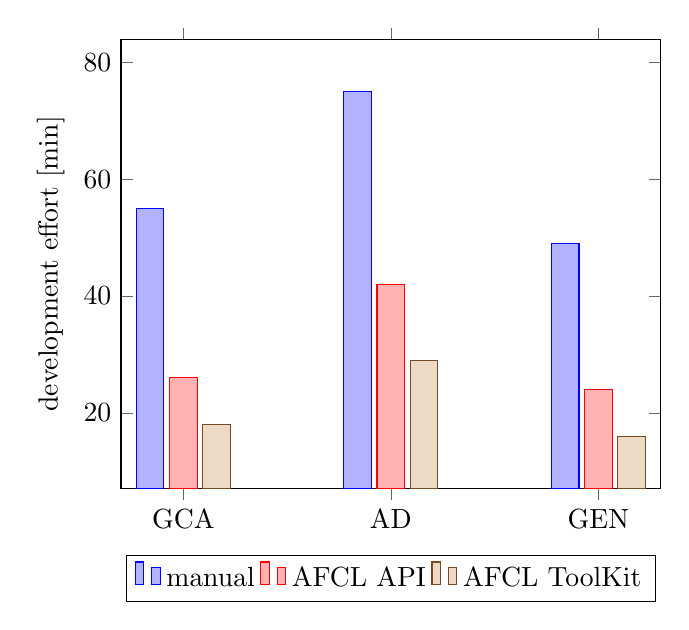
\begin{tikzpicture}
\begin{axis}[
    ybar,
    enlargelimits=0.15,
    legend style={at={(0.5,-0.15)},
      anchor=north,legend columns=-1},
    ylabel={development effort [min]},
    symbolic x coords={GCA,AD,GEN},
    xtick=data,
    nodes near coords align={vertical},
    ]
\addplot coordinates {(GCA,55) (AD,75) (GEN,49)};
\addplot coordinates {(GCA,26) (AD,42) (GEN,24)};
\addplot coordinates {(GCA,18) (AD,29) (GEN,16)};
\legend{manual,AFCL API,AFCL ToolKit}
\end{axis}
\end{tikzpicture}
\caption{Evaluated development effort for creating GCA, AD and GEN AFCL FC using methods manual, AFCL API, AFCL ToolKit}
\label{fig:evaluation-composing}
\end{figure}

% toolkit has to insert functions first
% java has to set up a project with AFCL API JAR
In summary, using AFCL ToolKit speeds up the process for creating AFCL FCs significantly, while minimizing human errors. According to \cite{books-code-complete-mcconnell}, the error rate of a developer is between 1.5\% and 5\% on average.
With AFCL ToolKits' validation while creating an FC, this error rate is minimized even further.
In addition to speedup, a benefit of using AFCL ToolKit over the other methods is that anyone with knowledge about AFCL could create the FC, there is no need to be a programmer.\\

\section{Adapting FCs}
\label{sec:evaluation-adapting}

The full benefit of AFCL Toolkit can be seen in FC adaptation.
In this section, the effort required for doing an FC adaptation as described in section \ref{sec:backend-adaptation} is measured.

For this evaluation, it was sufficient to only measure the effort needed to divide one loop into two loops. Since the procedure would be the same for every additional loop, the total approximated effort can be determined by multiplying the effort which was needed for a divide into two loops, with the number of divides.
In the following, we will only consider the GCA FC example, since this includes one \texttt{ParallelFor} loop.
The effort is also dependent of the number of affected data elements in subsequent functions, which have to be adjusted. In the GCA FC, there are twelve data elements which need to be updated after a divide.

To divide the loop of the GCA FC into two loops, it took approximately 27 minutes using the manual method, approximately 12 minutes using the AFCL API and less than 1 minute using AFCL ToolKit. Figure \ref{fig:evaluation-adaptation} shows the development effort needed for a divide from one to five times.  

\clearpage

Since the only thing which has to be done manually when using AFCL ToolKit is basically load the FC and push a button, the speedup for this adaptation using AFCL ToolKit over the other two methods always approaches 99\%.

\begin{figure}[h]
\vspace{1.5cm}
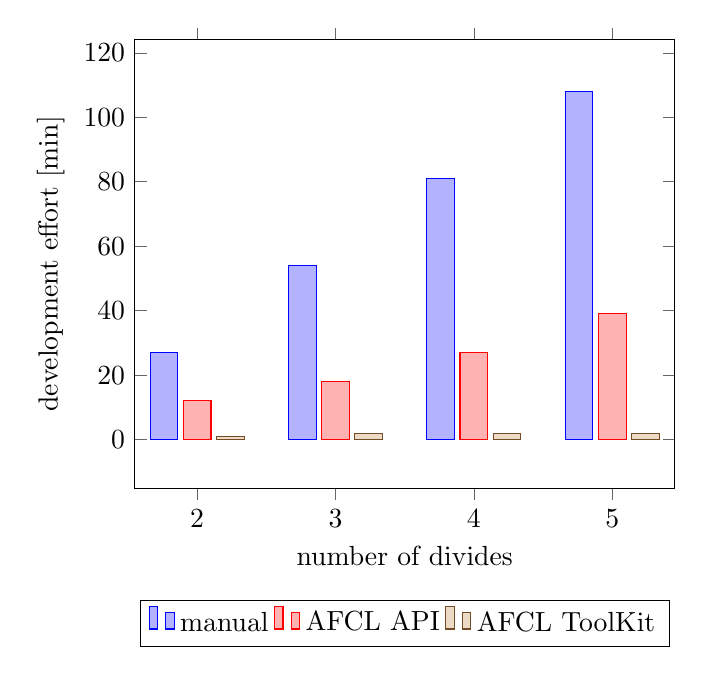
\begin{tikzpicture}
\begin{axis}[
    ybar,
    enlargelimits=0.15,
    legend style={at={(0.5,-0.25)},
      anchor=north,legend columns=-1},
    ylabel={development effort [min]},
    xlabel={number of divides},
    xtick=data,
    nodes near coords align={vertical},
    ]
\addplot coordinates {(2,27) (3,54) (4,81) (5,108)};
\addplot coordinates {(2,12) (3,18) (4,27) (5,39)};
\addplot coordinates {(2,1) (3,2) (4,2) (5,2)};
\legend{manual,AFCL API,AFCL ToolKit}
\end{axis}
\end{tikzpicture}
\caption{Evaluated development effort for adapting FCs using methods manual, AFCL API and AFCL ToolKit.}
\label{fig:evaluation-adaptation}
\end{figure}

% realistic example
% company average uses five clouds (paper/website ?)
% how much time would be needed to update manually
% maybe twenty gates will change for a bigger airport
% run multiple workflows each with big number of passengers
% with system update automatically workflows

\chapter{Discussion}
\label{chap:discussion}

Although simplifying the creation of FCs for non-developers was one of the primary goals of this work, a side product emerged during development, which simplifies creation and adaptation of FCs with the AFCL API.

The AFCL Java API in its current state focuses on creating AFCL compliant FCs by writing Java code. It provides classes which define function and control-structure objects, as well as data objects, each of them representing an AFCL construct. The objects can be arranged, connected and nested in a \texttt{Workflow}, in order to define execution flow. Data objects can be associated with functions or control-structure objects to define data-flow.

However, the API has limitations. One is that a \texttt{Function} does not have a reference to its \textit{parent object}. The \textit{parent object} can be either a \texttt{Workflow} or \texttt{Compound}, each with its own implementation how for accessing its enclosed functions - there is no common super class or interface that provides a method. The same problem occurs with \texttt{DataIns}, \texttt{DataOuts} and \texttt{DataOutsAtomic}, they do have properties (e.g. \texttt{source}) in common, but each of it has its own implementation for accessing them. This is also the case for \texttt{AtomicFunction} and \texttt{Compound} and the \texttt{dataIns} property.\\
Furthermore, tasks like iterating over all \texttt{Function} objects in a \texttt{Workflow} are not supported out of the box.

The above mentioned limitations make it challenging to perform automated modifications while keeping code generic.
During development, it turned out that the following tasks were used frequently when modifying an FC programmatically:

\clearpage

\begin{itemize}
    \item traverse a \texttt{Workflow}, in particular, iterate over all \texttt{Function} objects inside a \texttt{Workflow}
	\item get a \texttt{Function} by its name
	\item get the \textit{parent object} of a Function (\texttt{Workflow} or \texttt{Compound})
	\item get the \texttt{List} which contains a given \texttt{Function}
	\item get all \texttt{DataIns} and \texttt{DataOuts} which use a given \texttt{Function} as source
\end{itemize}

The implementation of this tasks has been achieved using a combination of generics and reflection, and can be found in \ref{apx:afcl-wrapper-functions}.

\chapter{Conclusion and Future Work}

With AFCL ToolKit, a system was developed that greatly simplifies the creation and adaptation of AFCL FCs. 
The implemented system fulfills the requirement of modeling FCs at a high level of abstraction by providing an editor where FCs can be created and edited in a WYSIWYG manner. It even goes further by providing additional user actions like a clipboard, versioning, auto-layout and validation, which make the creation process more convenient.
The system can also load existing AFCL FCs for visualization and further editing and supports three different formats for exporting FCs.

We have shown that the system with its benefits leads to an significant speedup for FC development and adaption.
With the implemented tool, AFCL is no longer reserved exclusively for developers - virtually anyone is able to develop an FC.

Despite AFCL ToolKit resulted in being a mostly final, ready-to-use product, it still can be further extended and improved.
Future work could include various improvements related to visualization, validation, user interaction or performance.\\
An improvement for usability could be a supportive validation for source fields when defining data-flow, for example by suggesting the available function names and data ports using autocomplete.
The representation of an FC could be clarified more by visualizing its data-flow, in interaction with the control flow.
Moreover, the information showed in tooltips when hovering graph nodes can be extended to show more details about the underlying user object.

\begin{appendix}


\chapter{AFCL API functions}
\label{apx:afcl-functions}

In the following paragraphs of this section, terms highlighted with a mono-spaced font refer to classes or class properties of the AFCL Java API.

The AFCL Java API in its current state provides classes which define function and control-structure objects, as well as data-flow objects of an AFCL workflow. They can be arranged and nested in a tree structure in order to model the execution flow.

However, the API has its limitations. One is that a \texttt{Function} does not have a reference to its \textit{parent object}. The \textit{parent object} can be either a \texttt{Workflow} or \texttt{Compound}, which has its own implementation to access its enclosed functions - there is no common super class or interface providing a common method. The same problem occurs on \texttt{DataIns}, \texttt{DataOuts} and \texttt{DataOutsAtomic}, they do have properties (e.g. \texttt{source}) in common, but each of them has its own implementation to access them. This is also the case for \texttt{AtomicFunction} and \texttt{Compound} and the \texttt{dataIns} property.\\
Furthermore, tasks like iterating over all \texttt{Function} objects in a \texttt{Workflow} are not supported. 

These limitations make it challenging to perform automated modifications while keep the code generic.
During development, it turned out that the following tasks were required frequently while modifying a workflow programmatically. We define these task  as \textit{general adaptation tasks}:
\begin{itemize}
	\item get a \texttt{Function} by its name
	\item get the \textit{parent object} of a Function (\texttt{Workflow} or \texttt{Compound})
	\item get the \texttt{List} which contains a given \texttt{Function}
	\item get all \texttt{DataIns} and \texttt{DataOuts} which use a given \texttt{Function} as source
	\item traverse a \texttt{Workflow}, in particular, iterate over all \texttt{Function} objects inside a \texttt{Workflow}
\end{itemize}

The generic requirement was achieved one the one hand by using \textit{Reflection}, on the other hand by developing a generic \textit{traverse function}, shown in listings \ref{lst:traverseWorkflow} and \ref{lst:traverseFunctions}.

\begin{lstlisting}[language=Java,caption={Traverse workflow},label={lst:traverseWorkflow}]
public static void traverseWorkflow(Workflow wf, BiConsumer<Function, Object> consumer) {
    traverseFunctions(wf.getWorkflowBody(), consumer, wf);
}
\end{lstlisting}

\begin{lstlisting}[language=Java,caption={Traverse functions},label={lst:traverseFunctions}]
public static void traverseFunctions(List<Function> functionsList, BiConsumer<Function, Object> consumer, Object currentParent) {
    if (functionsList == null) {
        return;
    }
    for (Function fn : functionsList) {
        consumer.accept(fn, currentParent);
        if (fn instanceof IfThenElse) {
            traverseFunctions(((IfThenElse) fn).getThen(), consumer, fn);
            traverseFunctions(((IfThenElse) fn).getElse(), consumer, fn);
        }
        if (fn instanceof Switch) {
            for (Case c : ((Switch) fn).getCases()) {
                traverseFunctions(c.getFunctions(), consumer, fn);
            }
        }
        if (fn instanceof Parallel) {
            for (Section s : ((Parallel) fn).getParallelBody()) {
                traverseFunctions(s.getSection(), consumer, fn);
            }
        }
        if (fn instanceof ParallelFor) {
            traverseFunctions(((ParallelFor) fn).getLoopBody(), consumer, fn);
        }
    }
}
\end{lstlisting}

As the reader may have noticed, the traverse function accepts Java's \texttt{BiConsumer} as second argument, which makes it very versatile in its usage. The given consumer operation - which can be a function reference or a lambda expression - is executed for every function element in the workflow, providing the element itself and its \textit{parent object} as arguments on traversal. This is indeed very powerful, reduces LOC, therefore improves readability, maintainability and efficiency. The only drawback is that all functions are always visited, because there is no proper way to break out of a lambda expression. There exist approaches to break out by throwing an Exception, however this is considered to be bad practice.

For example, getting a function by its name, can be achieved as showed in listing \ref{lst:getFuncByName}. \small Note that mutating variables in lamda expressions is not thread-safe, so an \texttt{AtomicReference} is used.

\begin{lstlisting}[language=Java,caption={get a function by its name},label=lst:getFuncByName]
final AtomicReference<Function> fRef = new AtomicReference<>();
traverseFunctions(fnList, (fn, parentObj) -> {
    if (fn.getName() != null && fn.getName().equals(name)) {
        fRef.set(fn);
    }
});
// do something with found function in fRef.get();
\end{lstlisting}

\end{appendix}

\printbibliography

\end{document}